\documentclass{article}

\usepackage{fancyhdr}
\usepackage{extramarks}
\usepackage{amsmath}
\usepackage{amsthm}
\usepackage{amsfonts}
\usepackage{tikz}
\usepackage[plain]{algorithm}
\usepackage{algpseudocode}
\usepackage{xcolor}
\usepackage{enumitem}
\usepackage{amssymb}
\usepackage{todonotes}
\usepackage{mathtools}
\usepackage{wasysym}
\usepackage{cancel}
\usepackage{phaistos}

\usetikzlibrary{automata,positioning}

%
% Basic Document Settings
%

\topmargin=-0.45in
\evensidemargin=0in
\oddsidemargin=0in
\textwidth=6.5in
\textheight=9.0in
\headsep=0.25in

\linespread{1.1}

\pagestyle{fancy}
\lhead{\hmwkAuthorName}
\chead{\hspace{2.5cm} \hmwkClass\ (\hmwkClassInstructor): \hmwkTitle}
\rhead{\firstxmark}
\lfoot{\lastxmark}
\cfoot{\thepage}

\renewcommand\headrulewidth{0.4pt}
\renewcommand\footrulewidth{0.4pt}

\setlength\parindent{0pt}

%
% Create Problem Sections
%

\newcommand{\enterProblemHeader}[1]{
    \nobreak\extramarks{}{Problem \arabic{#1} continued on next page\ldots}\nobreak{}
    \nobreak\extramarks{Problem \arabic{#1} (continued)}{Problem \arabic{#1} continued on next page\ldots}\nobreak{}
}

\newcommand{\exitProblemHeader}[1]{
    \nobreak\extramarks{Problem \arabic{#1}}{Problem \arabic{#1} continued on next page\ldots}\nobreak{}
    \stepcounter{#1}
    \nobreak\extramarks{Problem \arabic{#1}}{}\nobreak{}
}

\newcount\colveccount
\newcommand*\colvec[1]{
        \global\colveccount#1
        \begin{pmatrix}
        \colvecnext
}
\def\colvecnext#1{
        #1
        \global\advance\colveccount-1
        \ifnum\colveccount>0
                \\
                \expandafter\colvecnext
        \else
                \end{pmatrix}
        \fi
}

\setcounter{secnumdepth}{0}
\newcounter{partCounter}
\newcounter{homeworkProblemCounter}
\setcounter{homeworkProblemCounter}{1}
\nobreak\extramarks{Problem \arabic{homeworkProblemCounter}}{}\nobreak{}

%
% Homework Problem Environment
%
% This environment takes an optional argument. When given, it will adjust the
% problem counter. This is useful for when the problems given for your
% assignment aren't sequential. See the last 3 problems of this template for an
% example.
%
\newenvironment{homeworkProblem}[1][-1]{
    \ifnum#1>0
        \setcounter{homeworkProblemCounter}{#1}
    \fi
    \section{Problem \arabic{homeworkProblemCounter}}
    \setcounter{partCounter}{1}
    \enterProblemHeader{homeworkProblemCounter}
}{
    \exitProblemHeader{homeworkProblemCounter}
}

%
% Homework Details
%   - Title
%   - Due date
%   - Class
%   - Section/Time
%   - Instructor
%   - Author
%

\newcommand{\hmwkTitle}{Assignment 3}
\newcommand{\hmwkDueDate}{October 12, 2018}
\newcommand{\hmwkClass}{Probability \& Statistics}
\newcommand{\hmwkClassTime}{Fall Semester}
\newcommand{\hmwkClassInstructor}{Prof. D. Eynard}
\newcommand{\hmwkAuthorName}{\textbf{A. Romanelli} / \textbf{A. Vicini}}

%
% Title Page
%

\title{
    \vspace{2in}
    \textmd{\textbf{\hmwkClass:\ \hmwkTitle}}\\
    \normalsize\vspace{0.1in}\small{Due\ on\ \hmwkDueDate\ at 8:30am}\\
    \vspace{0.1in}\large{\textit{\hmwkClassInstructor}}
    \vspace{3in}
}

\author{\hmwkAuthorName}
\date{}

\renewcommand{\part}[1]{\textbf{\large Part \Alph{partCounter}}\stepcounter{partCounter}\\}

%
% Various Helper Commands
%

% Useful for algorithms
\newcommand{\alg}[1]{\textsc{\bfseries \footnotesize #1}}

% For derivatives
\newcommand{\deriv}[1]{\frac{\mathrm{d}}{\mathrm{d}x} (#1)}

% For partial derivatives
\newcommand{\pderiv}[2]{\frac{\partial}{\partial #1} (#2)}

% Integral dx
\newcommand{\dx}{\mathrm{d}x}

% Alias for the Solution section header
\newcommand{\solution}{\textbf{\large Solution}}

% Probability commands: Expectation, Variance, Covariance, Bias
\newcommand{\E}{\mathrm{E}}
\newcommand{\Var}{\mathrm{Var}}
\newcommand{\Cov}{\mathrm{Cov}}
\newcommand{\Bias}{\mathrm{Bias}}

\begin{document}

\maketitle

\pagebreak

\begin{homeworkProblem}
	In this lottery the odds will be against us. We expect our win to be the following: 
	$$E[X] := \sum_{x \in X} P_X(x)x$$
	In our case, this translates to the four different scenario, where we have four different values:
	$$(\text{probability of winning 50'000\$}\cdot 50'000\$) + (\text{probability of winning 1'000\$} \cdot 1000\$)$$$$ + (\text{probability of winning 500\$} \cdot 500\$) + (\text{probability of losing\$} \cdot 0\$)$$
	To each of this values though we will need to subtract the price we pay for a ticker, which we need to pay in any case.
	$$\frac1{10000}\cdot 49'990\$ + \frac2{10000}\cdot 990\$ + \frac3{10000}\cdot 490\$ + \frac{9994}{10000}\cdot (-10\$) \approx 5\$ + 0.2\$ + 0.15\$ - 10\$ \approx -4.65\$$$
	We can clearly see that the expected value is negative, it wouldn't be probabilistically convenient for us to purchase a ticket for this particular lottery.
\end{homeworkProblem}

\begin{homeworkProblem}
	\begin{enumerate}[label=\textbf{\alph*)}]
		\item We compute the sum of each face value times its probability, which yields us:
		$$\sum_{i = 1}^{12}p(i)i = p(i)\cdot \sum_{i=1}^{12}i = p(i) \cdot \frac{i\cdot (i+1)}2= p(i) \cdot \frac{12 \cdot 13}2 = \frac1{12} \cdot 78 = 6.5$$
		Since in the summation we always add $i$ multiplied for $p(i)$, which instead is constant in this case, we can just bring it out of the summation.
		\item We do the same as for the previous question, but this time computing two expected value of 1d4 multiply by 2 and of 1d6 and sum them together:
		$$2\cdot p(i)\sum_{i = 1}^4i + p(i)\sum_{ i = 1}^6i = 2\cdot\frac14\cdot10 + \frac16\cdot21 = 8.5$$
		\item For $X = 2$ we have a 
		$$\binom32 \cdot \frac1{28} = \frac3{28}$$ chances of extracting two defective light bulbs. \\ 
		Whereas for $X = 1$, we have 
		$$\binom31 \cdot \binom51 \cdot \frac1{28} = \frac{3!}{2!1!} \cdot \frac{5!}{4!1!} \cdot \frac1{28} = 3 \cdot 5 \cdot \frac1{28} = \frac{15}{28}$$
		chances of finding a defective and a working bulb. \\
		Finally for $X = 0$ we get a $$\binom52 \cdot \frac1{28} = \frac{10}{28}$$ chances of finding two working light bulbs. \\ 
		$$E[X] = \frac3{28}\cdot 2 + \frac{10}{28} \cdot 1 + 0 = \frac6{28} + \frac{15}{28} = \frac34 = 0.75 $$
	\end{enumerate}
\end{homeworkProblem}
\newpage
\begin{homeworkProblem}
	\paragraph{a)}
	\begin{center}
		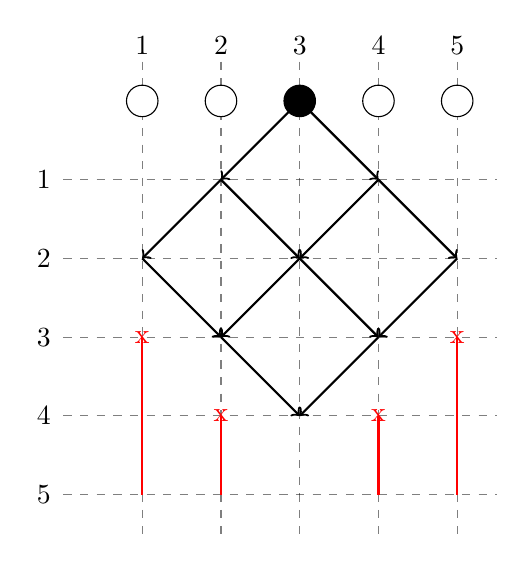
\begin{tikzpicture}
			\draw[->, thick] (3,-0.5) -- (2,-1.5);
			\draw[->, thick] (3,-0.5) -- (4,-1.5);
			
			\draw[->, thick] (2,-1.5) -- (1,-2.5);
			\draw[->, thick] (2,-1.5) -- (3,-2.5);
			\draw[->, thick] (4,-1.5) -- (3,-2.5);
			\draw[->, thick] (4,-1.5) -- (5,-2.5);
			
			\draw[->, thick] (3,-2.5) -- (2,-3.5);
			\draw[->, thick] (3,-2.5) -- (4,-3.5);
			\draw[->, thick] (5,-2.5) -- (4,-3.5);
			\draw[->, thick] (1,-2.5) -- (2,-3.5);
			
			
			\draw[->, thick] (2,-3.5) -- (3,-4.5);
			\draw[->, thick] (4,-3.5) -- (3,-4.5);
			\foreach \i in {1,...,5} {
				\draw[style=dashed, opacity=0.5] (\i, 0) -- (\i,-6);
				\draw[style=dashed, opacity=0.5] (0, -\i-0.5) -- (5.5, -\i-0.5);
				\node at (\i,0+0.2) {\i};
				\node at (-0.25, -\i-0.5) {\i};
				\fill[fill=white, draw=black] (\i, -0.5) circle (2mm);
			}
			\fill (3, -0.5) circle (2mm);
			\node at (1,-3.5) {\color{red}x};
			\node at (2,-4.5) {\color{red}x};
			\node at (5,-3.5) {\color{red}x};
			\node at (4,-4.5) {\color{red}x};			
			\draw[color=red, thick] (1,-3.5) -- (1, -5.5);
			\draw[color=red, thick] (2,-4.5) -- (2, -5.5);
			\draw[color=red, thick] (5,-3.5) -- (5, -5.5);
			\draw[color=red, thick] (4,-4.5) -- (4, -5.5);			
		\end{tikzpicture}
	\end{center}
	If the coin is handed out to $p_3$ it would take us 3 passes to be certain that $p_1$ and $p_5$ do not possess the coin and we could eliminate them from the process, leaving us with $p_2, p_3$ and $p_4$. The next pass of the coins will ensure that the coin is back to $p_3$, thus eliminating $p_2$ and $p_4$ only leaves us with $p_3$ which is where the coin currently is.
	\paragraph{b)}
		\begin{center}
		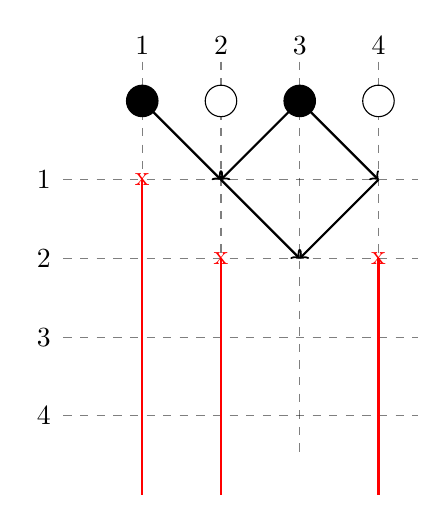
\begin{tikzpicture}
			\draw[->, thick] (3,-0.5) -- (2,-1.5);
			\draw[->, thick] (3,-0.5) -- (4,-1.5);
			
			\draw[->, thick] (1,-0.5) -- (2,-1.5);
			\draw[->, thick] (2,-1.5) -- (3,-2.5);
			\draw[->, thick] (4,-1.5) -- (3,-2.5);
			
			
			\foreach \i in {1,...,4} {
				\draw[style=dashed, opacity=0.5] (\i, 0) -- (\i,-5);
				\draw[style=dashed, opacity=0.5] (0, -\i-0.5) -- (4.5, -\i-0.5);
				\node at (\i,0+0.2) {\i};
				\node at (-0.25, -\i-0.5) {\i};
				\fill[fill=white, draw=black] (\i, -0.5) circle (2mm);
			}
			\fill (3, -0.5) circle (2mm);
			\fill (1, -0.5) circle (2mm);
			\node at (1,-1.5) {\color{red}x};
			\node at (2,-2.5) {\color{red}x};
			\node at (4,-2.5) {\color{red}x};			
			\draw[color=red, thick] (1,-1.5) -- (1, -5.5);
			\draw[color=red, thick] (2,-2.5) -- (2, -5.5);
			\draw[color=red, thick] (4,-2.5) -- (4, -5.5);			
		\end{tikzpicture}
	\end{center}
	We can give the coin to $p_1$ or $p_3$, and after we've passed the coin once we can remove $p_1$, which leaves us with the other three people. The next pass that will be performed will ensure us that the coin will be back to $p_3$ and the same strategy is applicable giving the coin to $p_2$ or $p_4$ and mirroring the process, removing $p_4$. 
\end{homeworkProblem}
\newpage
\begin{homeworkProblem}
	The trick we used earlier bases its reliability on the fact that we have some boundaries: these are given by the fact that the five people of \textbf{Problem 3, Question a)} were put on a row. As a consequence, the people whose position lies on the outer side \textemdash\ initially 1 and 5 \textemdash can only pass the coin back, effectively bouncing back the coin. This bouncing back would then make us sure that the odds of having the coin converged on the inner people, which allowed us to exclude 1 and 5. \\ \\
	This strategy is not applicable in this context because of the circular disposition of the participants. If the disposition of the participants is a circle, it means that there can be no boundaries on where the coin goes and we cannot force it to converge anywhere, thus no participant can be taken out. \\ \\
	Example with odd number of participants:
	\begin{center}
		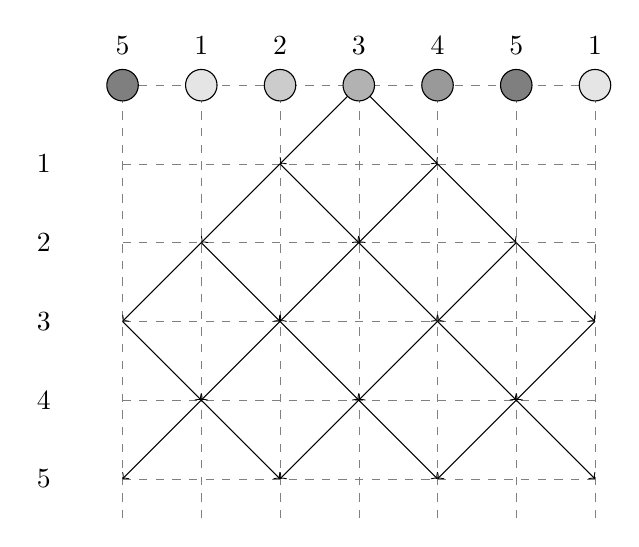
\begin{tikzpicture}
		
		
			\draw[step=1cm,gray,very thin,dashed] (0.,-1) grid (6,-6.5);
			
			\draw[->] (3,-1) -- (2,-2);
			\draw[->] (3,-1) -- (4,-2);	
			
			\draw[->] (2,-2) -- (3,-3);
			\draw[->] (2,-2) -- (1,-3);	
			\draw[->] (4,-2) -- (3,-3);
			\draw[->] (4,-2) -- (5,-3);	
			
			\draw[->] (3,-3) -- (2,-4);
			\draw[->] (3,-3) -- (4,-4);			
			\draw[->] (1,-3) -- (0,-4);
			\draw[->] (1,-3) -- (2,-4);			
			\draw[->] (5,-3) -- (4,-4);
			\draw[->] (5,-3) -- (6,-4);
			
			\draw[->] (2,-4) -- (1,-5);
			\draw[->] (2,-4) -- (3,-5);
			\draw[->] (4,-4) -- (3,-5);
			\draw[->] (4,-4) -- (5,-5);
			\draw[->] (0,-4) -- (1,-5);
			\draw[->] (6,-4) -- (5,-5);
			
			\draw[->] (1,-5) -- (0,-6);
			\draw[->] (1,-5) -- (2,-6);
			\draw[->] (3,-5) -- (2,-6);
			\draw[->] (3,-5) -- (4,-6);
			\draw[->] (5,-5) -- (4,-6);
			\draw[->] (5,-5) -- (6,-6);
			
						
									
			\fill[fill=white, draw=black] (0, -1) circle (2mm);
				\node at (0,-0.5) {5};
			\fill[fill=white, draw=black] (6, -1) circle (2mm);
			\node at (6,-0.5) {1};
			
			
			\foreach \i in {1,...,5} {
%				\draw[style=dashed, opacity=0.5] (\i, 0) -- (\i,-6);
%				\draw[style=dashed, opacity=0.5] (0, -\i-0.5) -- (5.5, -\i-0.5);
				\node at (\i,-0.5) {\i};
				\node at (-1, -\i-1) {\i};
				\fill[fill=white, draw=black] (\i, -1) circle (2mm);
			}
				
			
			
			\fill[opacity=0.5] (0, -1) circle (2mm);
			\fill[opacity=0.1] (1, -1) circle (2mm);
			\fill[opacity=0.2] (2, -1) circle (2mm);
			\fill[opacity=0.3] (3, -1) circle (2mm);
			\fill[opacity=0.4] (4, -1) circle (2mm);
			\fill[opacity=0.5] (5, -1) circle (2mm);
			\fill[opacity=0.1] (6, -1) circle (2mm);


		\end{tikzpicture}
	\end{center}
	We can see as always that every time we pass a coin the odds switch from the odd-numbered participants to the even-numbered one, thus we could keep count of the moves done and remove either the odd-numbered or the even-numbered, in the first case we'd be left with an 2 choices in this case with an equal amount of probability, which doesn't work for us. In the other case it would leave us with 3 choices:
	
	\begin{center}
		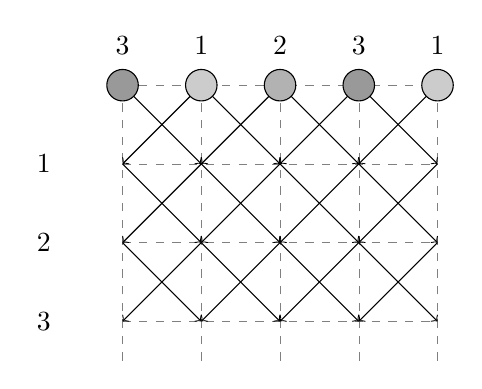
\begin{tikzpicture}
		
		
			\draw[step=1cm,gray,very thin,dashed] (0.,-1) grid (4,-4.5);
			
			\draw[->] (0,-1) -- (1,-2);
			
			\draw[->] (1,-1) -- (2,-2);
			\draw[->] (1,-1) -- (0,-2);
				
			\draw[->] (2,-1) -- (1,-2);
			\draw[->] (2,-1) -- (3,-2);	
			
			\draw[->] (3,-1) -- (2,-2);
			\draw[->] (3,-1) -- (4,-2);
			
			\draw[->] (4,-1) -- (3,-2);
			
			\draw[->] (0,-2) -- (1,-3);
			
			\draw[->] (1,-2) -- (2,-3);
			\draw[->] (1,-2) -- (0,-3);
				
			\draw[->] (2,-2) -- (1,-3);
			\draw[->] (2,-2) -- (3,-3);	
			
			\draw[->] (3,-2) -- (2,-3);
			\draw[->] (3,-2) -- (4,-3);
			
			\draw[->] (4,-2) -- (3,-3);
			
			\draw[->] (0,-3) -- (1,-4);
			
			\draw[->] (1,-3) -- (2,-4);
			\draw[->] (1,-3) -- (0,-4);
				
			\draw[->] (2,-3) -- (1,-4);
			\draw[->] (2,-3) -- (3,-4);	
			
			\draw[->] (3,-3) -- (2,-4);
			\draw[->] (3,-3) -- (4,-4);
			
			\draw[->] (4,-3) -- (3,-4);			
						
			\fill[fill=white, draw=black] (0, -1) circle (2mm);
			\node at (0,-0.5) {3};
			\fill[fill=white, draw=black] (4, -1) circle (2mm);
			\node at (4,-0.5) {1};
						
			\foreach \i in {1,...,3} {
				\node at (\i,-0.5) {\i};
				\node at (-1, -\i-1) {\i};
				\fill[fill=white, draw=black] (\i, -1) circle (2mm);
			}
				
			
			
			\fill[opacity=0.4] (0, -1) circle (2mm);
			\fill[opacity=0.2] (1, -1) circle (2mm);
			\fill[opacity=0.3] (2, -1) circle (2mm);
			\fill[opacity=0.4] (3, -1) circle (2mm);
			\fill[opacity=0.2] (4, -1) circle (2mm);


		\end{tikzpicture}
	\end{center}
	But at this point, our newly established 1, 2 and 3 have all the same chance of having the coin at this point, which is the same as starting the game with only these three participants and randomly giving them a coin. We won't be able to be sure about who possess the coin because we wouldn't know where we started from. \\ \\
	Thus there can't be a viable strategy that ensures us to know which participant will hold the coin.
\end{homeworkProblem}
\end{document}
